\documentclass{beamer}
\usepackage{amsmath}
\usepackage[english]{babel} %set language; note: after changing this, you need to delete all auxiliary files to recompile
\usepackage[utf8]{inputenc} %define file encoding; latin1 is the other often used option
\usepackage{csquotes} % provides context sensitive quotation facilities
\usepackage{graphicx} %allows for inserting figures
\usepackage{booktabs} % for table formatting without vertical lines
\usepackage{textcomp} % allow for example using the Euro sign with \texteuro
\usepackage{stackengine}
\usepackage{wasysym}
\usepackage{tikzsymbols}
\usepackage{textcomp}
\usepackage{xcolor}
\usepackage[dvipsnames]{xcolor}
\usepackage{colortbl}
\usepackage{adjustbox}
\newcommand{\bubblethis}[2]{
        \tikz[remember picture,baseline]{\node[anchor=base,inner sep=0,outer sep=0]%
        (#1) {\underline{#1}};\node[overlay,cloud callout,callout relative pointer={(0.2cm,-0.7cm)},%
        aspect=2.5,fill=yellow!90] at ($(#1.north)+(-0.5cm,1.6cm)$) {#2};}%
    }%
\tikzset{face/.style={shape=circle,minimum size=4ex,shading=radial,outer sep=0pt,
        inner color=white!50!yellow,outer color= yellow!70!orange}}
%% Some commands to make the code easier
\newcommand{\emoticon}[1][]{%
  \node[face,#1] (emoticon) {};
  %% The eyes are fixed.
  \draw[fill=white] (-1ex,0ex) ..controls (-0.5ex,0.2ex)and(0.5ex,0.2ex)..
        (1ex,0.0ex) ..controls ( 1.5ex,1.5ex)and( 0.2ex,1.7ex)..
        (0ex,0.4ex) ..controls (-0.2ex,1.7ex)and(-1.5ex,1.5ex)..
        (-1ex,0ex)--cycle;}
\newcommand{\pupils}{
  %% standard pupils
  \fill[shift={(0.5ex,0.5ex)},rotate=80] 
       (0,0) ellipse (0.3ex and 0.15ex);
  \fill[shift={(-0.5ex,0.5ex)},rotate=100] 
       (0,0) ellipse (0.3ex and 0.15ex);}

\newcommand{\emoticonname}[1]{
  \node[below=1ex of emoticon,font=\footnotesize,
        minimum width=4cm]{#1};}
\usepackage{scalerel}
\usetikzlibrary{positioning}
\usepackage{xcolor,amssymb}
\newcommand\dangersignb[1][2ex]{%
  \scaleto{\stackengine{0.3pt}{\scalebox{1.1}[.9]{%
  \color{red}$\blacktriangle$}}{\tiny\bfseries !}{O}{c}{F}{F}{L}}{#1}%
}
\newcommand\dangersignw[1][2ex]{%
  \scaleto{\stackengine{0.3pt}{\scalebox{1.1}[.9]{%
  \color{red}$\blacktriangle$}}{\color{white}\tiny\bfseries !}{O}{c}{F}{F}{L}}{#1}%
}
\usepackage{fontawesome} % Social Icons
\usepackage{epstopdf} % allow embedding eps-figures
\usepackage{tikz} % allows drawing figures
\usepackage{amsmath,amssymb,amsthm} %advanced math facilities
\usepackage{lmodern} %uses font that support italic and bold at the same time
\usepackage{hyperref}
\usepackage{tikz}
\hypersetup{
    colorlinks=true,
    linkcolor=blue,
    filecolor=magenta,      
    urlcolor=blue,
}
\usepackage{tcolorbox}
%add citation management using BibLaTeX
\usepackage[citestyle=authoryear-comp, %define style for citations
    bibstyle=authoryear-comp, %define style for bibliography
    maxbibnames=10, %maximum number of authors displayed in bibliography
    minbibnames=1, %minimum number of authors displayed in bibliography
    maxcitenames=3, %maximum number of authors displayed in citations before using et al.
    minnames=1, %maximum number of authors displayed in citations before using et al.
    datezeros=false, % do not print dates with leading zeros
    date=long, %use long formats for dates
    isbn=false,% show no ISBNs in bibliography (applies only if not a mandatory field)
    url=false,% show no urls in bibliography (applies only if not a mandatory field)
    doi=false, % show no dois in bibliography (applies only if not a mandatory field)
    eprint=false, %show no eprint-field in bibliography (applies only if not a mandatory field)
    backend=biber %use biber as the backend; backend=bibtex is less powerful, but easier to install
    ]{biblatex}
\addbibresource{../mybibfile.bib} %define bib-file located one folder higher


\usefonttheme[onlymath]{serif} %set math font to serif ones

\definecolor{beamerblue}{rgb}{0.2,0.2,0.7} %define beamerblue color for later use

%%% defines highlight command to set text blue
\newcommand{\highlight}[1]{{\color{blue}{#1}}}


%%%%%%% commands defining backup slides so that frame numbering is correct

\newcommand{\backupbegin}{
   \newcounter{framenumberappendix}
   \setcounter{framenumberappendix}{\value{framenumber}}
}
\newcommand{\backupend}{
   \addtocounter{framenumberappendix}{-\value{framenumber}}
   \addtocounter{framenumber}{\value{framenumberappendix}}
}

%%%% end of defining backup slides

%Specify figure caption, see also http://tex.stackexchange.com/questions/155738/caption-package-not-working-with-beamer
\setbeamertemplate{caption}{\insertcaption} %redefines caption to remove label "Figure".
%\setbeamerfont{caption}{size=\scriptsize,shape=\itshape,series=\bfseries} %sets figure  caption bold and italic and makes it smaller


\usetheme{Boadilla}

%set options of hyperref package
\hypersetup{
    bookmarksnumbered=true, %put section numbers in bookmarks
    naturalnames=true, %use LATEX-computed names for links
    citebordercolor={1 1 1}, %color of border around cites, here: white, i.e. invisible
    linkbordercolor={1 1 1}, %color of border around links, here: white, i.e. invisible
    colorlinks=true, %color links
    anchorcolor=black, %set color of anchors
    linkcolor=beamerblue, %set link color to beamer blue
    citecolor=blue, %set cite color to beamer blue
    pdfpagemode=UseThumbs, %set default mode of PDF display
    breaklinks=true, %break long links
    pdfstartpage=1 %start at first page
    }

\newtcolorbox{boxA}{
    fontupper = \bf,
    boxrule = 1.5pt,
    colframe = black % frame color
}
\newtcolorbox{boxB}{
    boxrule = 1.5pt,
    colframe = blue!70!black,, % frame color
    colback = blue!7!white,
}

% --------------------
% Overall information
% --------------------
\title[Economía I]{Economía I \vspace{3mm}
\\ Magistral 18 \vspace{3mm} \\ Introducción a la Macroeconomía}
\date{}
\author[Victoria Rosino]{Victoria Rosino}
\vspace{0.3cm}
\institute[]{Universidad de San Andrés} 

\begin{document}

\begin{frame}
\vspace{0.3cm}
\titlepage
\centering
\vspace{-0.9cm}
\includegraphics[scale=0.3]{Slides Principios de Economia/Figures/udesa_logo.jpg} 
\end{frame}

\begin{frame}{Las grandes preguntas de la macroeconomía}
    \begin{itemize}
        \item ¿Por qué la economía vive ciclos de expansión y de recesión?
        \item ¿Qué determina el nivel agregado de producción?
        \item ¿Qué determina el crecimiento de largo plazo?
        \item ¿Por qué hay inflación en algunos países?
        \item ¿Qué pasa cuando el Estado interviene en la economía?
    \end{itemize} 
    
\end{frame}


\begin{frame}
\frametitle{Evaluando toda la economía}
\begin{itemize}
        \item Para evaluar cómo una persona está en términos económicos solemos mirar sus ingresos \vspace{1mm}
        \item Para una economía hacemos lo mismo, pero una economía es un sistema en el que diversos agentes interactúan: \vspace{1mm}
        \begin{itemize}
            \item Hogares
            \item Empresas
            \item Instituciones financieras
            \item Gobierno
            \item Sector externo
        \end{itemize}
\end{itemize}
\end{frame}

\begin{frame}{Flujo circular de la riqueza (cerrado)}
    \begin{figure} [H]
\centering
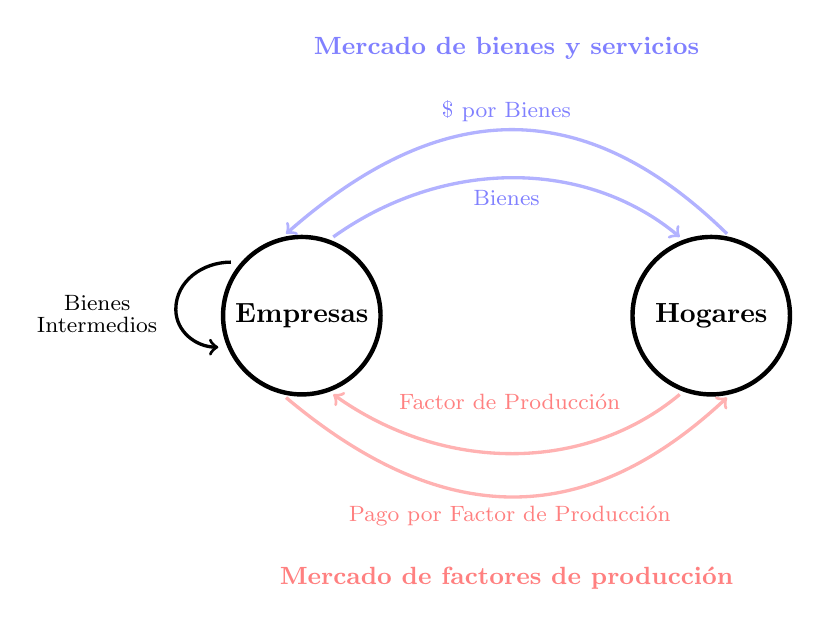
\begin{tikzpicture}[scale=0.4]
\node[blue!50] at (8.5,8.5) {\small \textbf{Mercado de bienes y servicios}};
\draw[ultra thick](2,0) circle [radius =2.5];
\node[] at (2,0) { \textbf{Empresas}};
\draw[ultra thick](15,0) circle [radius =2.5];
\node[] at (15,0) {\textbf{Hogares} };
\draw [very thick, ->] (-0.25, 1.7) to [out=-180, in=90] (-2, 0.2) to [out=-90, in=180] (-0.65, -1);
\node[] at (-4.5,0.4) {\footnotesize  Bienes};
\node[] at (-4.5,-0.3) {\footnotesize  Intermedios};
\draw[very thick, ->, blue!30] (3,2.5).. controls (6.5,5) and (11,5) .. (14,2.5);
\draw[very thick, <-, blue!30] (1.5,2.6).. controls (6.5,7) and (11,7) .. (15.5,2.6);
\node[blue!50] at (8.5,3.75) {\footnotesize  Bienes};
\node[blue!50] at (8.5,6.5) {\footnotesize  \$ por Bienes};
\draw[very thick, <-, red!30] (3,-2.5).. controls (6.5,-5) and (11,-5) .. (14,-2.5);
\draw[very thick, ->, red!30] (1.5,-2.6).. controls (6.5,-6.8) and (11,-6.8) .. (15.5,-2.6);
\node[red!50] at (8.6,-2.75) {\footnotesize  Factor de Producción};
\node[red!50] at (8.6,-6.35) {\footnotesize Pago por Factor de Producción};
\node[red!50] at (8.5,-8.35) {\small \textbf{Mercado de factores de producción}};
\end{tikzpicture}
\label{fig:25.1}
\end{figure} 

\end{frame}


\begin{frame}{Definiendo el PBI}
    \begin{boxB}
    \centering
        El PBI se define como el valor de mercado del conjunto de bienes y servicios finales que se produce en una economía en un determinado período de tiempo.
    \end{boxB}
\begin{itemize}
\vspace{2mm}
   \item En términos del gráfico del flujo circular, el PBI correspondería al conjunto de transacciones que se realizan en la rama superior (los productos finales que las firmas venden a los hogares). \vspace{1mm}
   \item  Pero a la vez, noten que la suma del valor de los bienes es igual a la suma de los ingresos! $\rightarrow$ el dinero que reciben los hogares por la rama inferior es la que gastan en la superior. \vspace{1mm}
   \item Por eso a veces nos referimos al PBI como ingreso nacional o doméstico.
   \end{itemize}
\end{frame}

\begin{frame}{Definiendo el PBI}
    \begin{boxB}
    \centering
        El PBI se define como el valor de mercado del conjunto de bienes y servicios finales que se produce en una economía en un determinado período de tiempo.
    \end{boxB}
\vspace{2mm}
Tres observaciones sobre la definición del PBI:
\begin{enumerate}
    \item Considera bienes y servicios \textbf{finales}: no se cuentan bienes intermedios
    \item Considera bienes y servicios \textbf{producidos en una economía}: importa que se produzcan en el país, no si corresponde a residentes o no residentes. \\
     \footnotesize - El Producto Bruto Nacional (PBN) es el indicador que considera únicamente la parte del PBI que le corresponde a los residentes del país.
    \item En un \textbf{periodo de tiempo}: la venta de un objeto preexistente no corresponde al concepto del PBI, es solo una transferencia de la propiedad de ese bien. 
\end{enumerate}

\end{frame}


\begin{frame}{Midiendo el PBI}
\vspace{2mm}
Tenemos tres maneras de medir el PBI: \vspace{1mm}
 \small
    \begin{enumerate}
    \item Por el gasto (valor de los bienes finales consumidos)
    \item Por los ingresos (suma de los ingresos recibidos) 
    \item Por el valor agregado (suma de los valores agregados en cada etapa de la producción)
    \end{enumerate}

    \vspace{3mm}
\begin{minipage}{0.47\textwidth}
\begin{table}[H]
\footnotesize
\begin{tabular}{cclc}
\rowcolor{blue!20}
\multicolumn{4}{c}{Agricultor} \\
\multicolumn{2}{c|}{\textbf{Ingresos}} & \multicolumn{2}{c}{\textbf{Costos}} \\ \hline
Harinas & \multicolumn{1}{c|}{300} & Salarios   & 800      \\
Huevos  & \multicolumn{1}{c|}{600} &      &   \\ \hline
& \multicolumn{1}{c|}{}  & \textbf{Beneficios} & \textbf{100} \\ 
\multicolumn{4}{c}{} \\
\end{tabular}
\end{table}
\end{minipage}
\hfill
\begin{minipage}{0.47\textwidth}
\begin{table}[H]
\footnotesize
\begin{tabular}{lclc}
\rowcolor{blue!20}
\multicolumn{4}{c}{Panadería} \\
\multicolumn{2}{c|}{\textbf{Ingresos}} & \multicolumn{2}{c}{\textbf{Costos}} \\ \hline
Pan  & \multicolumn{1}{c|}{900}  & Salarios   & 500   \\
Tortas & \multicolumn{1}{c|}{1000} & Harina  & 300 \\
\multicolumn{1}{l}{} & \multicolumn{1}{l|}{}     & \multicolumn{1}{l}{Huevos} & \multicolumn{1}{l}{600} \\ \hline
& \multicolumn{1}{c|}{}  & \textbf{Beneficios}  & \textbf{500}                  \end{tabular}
\end{table}
\end{minipage}
 \vspace{-3mm}
\begin{enumerate}
\footnotesize
    \item \textbf{Gasto (bienes finales)}: $PBI = 900+1000=1900$ 
    \item \textbf{Ingresos}: $PBI=$ Salarios + Beneficios = $1300 +600 =1900$ 
    \item \textbf{Valor agregado}: $PBI= VA_{ag}+VA_p=(900-0)+(1900-900)=1900$ 
\end{enumerate}
\end{frame}


\begin{frame}
\frametitle{Otros elementos importantes}
\begin{itemize}
        \item ¿Cómo incorporamos el sector externo?
        \begin{itemize}
        \item Como el PBI mide la \textbf{producción dentro del país}, debemos \textbf{incluir las exportaciones} (producción nacional que se consume en el extranjero), pero \textbf{excluir la importaciones} (producción extranjera que se consume internamente).
        \end{itemize} \vspace{1mm}
        \item ¿Cómo incorporamos al gobierno?
        \begin{itemize}
            \item Se lo trata básicamente como otro productor.
            \item Los bienes públicos son “comprados” con impuestos y se los valua por el costo de producirlos o brindarlos.
            \end{itemize}
\end{itemize}
\end{frame}


\begin{frame}
\frametitle{Sector externo}
\begin{figure} [H]
\centering
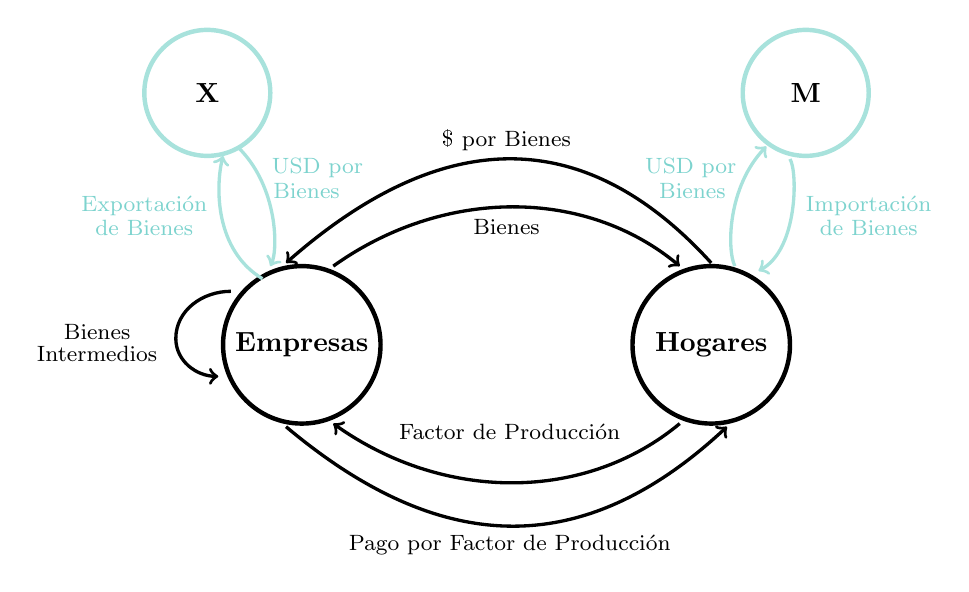
\begin{tikzpicture}[scale=0.4]
\draw[ultra thick](2,0) circle [radius =2.5];
\node[] at (2,0) { \textbf{Empresas}};
\draw[ultra thick](15,0) circle [radius =2.5];
\node[] at (15,0) { \textbf{Hogares} };
\draw[ultra thick, BlueGreen!40](18,8) circle [radius =2];
\node[] at (18,8) { \textbf{M}};
\draw[ultra thick, BlueGreen!40](-1,8) circle [radius =2];
\node[] at (-1,8) {\textbf{X}};
\draw [very thick, ->] (-0.25, 1.7) to [out=-180, in=90] (-2, 0.2) to [out=-90, in=180] (-0.65, -1);
\node[] at (-4.5,0.4) { \footnotesize Bienes};
\node[] at (-4.5,-0.3) {\footnotesize  Intermedios};
\draw[very thick, ->, ] (3,2.5).. controls (6.5,5) and (11,5) .. (14,2.5);
\draw[very thick, <-, ] (1.5,2.6).. controls (6.5,7) and (11,7) .. (15,2.6);
\node[] at (8.5,3.75) {\footnotesize  Bienes};
\node[] at (8.5,6.5) {\footnotesize  \$ por Bienes};
\draw[very thick, <-, ] (3,-2.5).. controls (6.5,-5) and (11,-5) .. (14,-2.5);
\draw[very thick, ->, ] (1.5,-2.6).. controls (6.5,-6.8) and (11,-6.8) .. (15.5,-2.6);
\node[] at (8.6,-2.75) { \footnotesize Factor de Producción};
\node[] at (8.6,-6.35) {\footnotesize Pago por Factor de Producción};
\draw[very thick, <-, BlueGreen!40] (1,2.5).. controls (1.25,3) and (1.25,5) .. (0,6.25);
\draw[very thick, ->, BlueGreen!40] (0.75,2.1).. controls (-0.75,3) and (-0.75,5) .. (-0.5,6);
\draw[very thick, <-, BlueGreen!40] (16.5,2.35).. controls (17.75,3) and (17.75,5.5) .. (17.5,5.9);
\draw[very thick, ->, BlueGreen!40] (15.75,2.5).. controls (15.5,3) and (15.5,5) .. (16.75,6.3);
\node[BlueGreen!60] at (-3,4.4) {\footnotesize  Exportación};
\node[BlueGreen!60] at (-3,3.7) {\footnotesize  de Bienes};
\node[BlueGreen!60] at (2.5,5.6) {\footnotesize  USD por};
\node[BlueGreen!60] at (2.15,4.9) {\footnotesize  Bienes};
\node[BlueGreen!60] at (20,4.4) {\footnotesize  Importación};
\node[BlueGreen!60] at (20,3.7) {\footnotesize  de Bienes};
\node[BlueGreen!60] at (14.35,5.6) {\footnotesize  USD por};
\node[BlueGreen!60] at (14.4,4.9) {\footnotesize  Bienes};
\end{tikzpicture}
\end{figure} 
\end{frame}

%\begin{frame}{Graficando el PBI de EEUU a largo plazo}
%    \begin{figure} [H]   \includegraphics[scale=1]{Slides Principios de Economia/Figures/G2.png}
%\end{figure}
%\end{frame}

%\begin{frame}{Ajustando con logs}
%    \begin{center}
%\begin{figure}[H]
%\renewcommand{\figurename}{Figure}
%\begin{center}
%    \begin{minipage}[b]{0.35\textwidth}
%        \begin{center}
%\begin{tikzpicture}[scale=0.4]
%\draw[very thick,<->] (0,11) node[left]{$f$}--(0,0)--(11,0) node[below]{$x$};
%\draw[semithick] (0,1).. controls (3,1) and (8, 1.1) .. (8.5, 8) node [right]{\footnotesize $Ae^{\lambda x}$};
%\end{tikzpicture}
%\end{center}
%     \end{minipage}
  %  \hfill
    %\begin{minipage}[b]{0.4\textwidth}
    %\begin{center}
%\begin{tikzpicture}[scale=0.35]
%\draw[very thick,<->] (0,11) node[left]{$f$}--(0,0)--(11,0) node[below]{$x$};
%\draw[semithick] (0,2)--(9, 7) node [right]{\footnotesize $log(Ae^{\lambda x})$};
%\draw[semithick, gray] (1,2.5)--(2,2.5)--(2,3.1);
%\node[] at (1.6,2) {\scriptsize $\lambda$};
%\node[left] at (0,2) {\footnotesize $log(A)$};
%\node[] at (11,6) {\footnotesize $=$};
%\node[] at (10.75,5.25) {\footnotesize $log(A)+\lambda x$};
%\end{tikzpicture}
%\end{center}
%    \end{minipage}
%\end{center}
%\end{figure}
%\end{center} 
%\end{frame}

%\begin{frame}{Re-graficando el PBI de EEUU a largo plazo en logs}
%   \begin{figure} [H]   \includegraphics[scale=0.45]{Slides Principios de Economia/Figures/C16.4.jpg}
%\end{figure}
%Fuente: \href{https://www.measuringworth.com/graphs/}{www.measuringworth.com}
%\end{frame}

\begin{frame}{PBI Nominal y Real}
    \begin{itemize}
        \item Considerar variables a \textit{valor de mercado} implica hacerlo a su precio\dots
        \item El PBI entonces es la suma de los bienes finales producidos a los precios de cada momento:
        \begin{equation*}
            PBI_{\text{NOMINAL}}^t = p_1^t q_1^t + p_2^t q_2^t + \cdots + p_N^t q_N^t.
        \end{equation*}
        \item Pero los precios cambian, por lo que el PBI nominal no es una buena medida de la producción real\dots
        \item Al PBI real lo vamos a definir como la suma de los bienes finales producidos en un año, pero valuados a los {\textcolor{blue}{precios de un año base}}:
        \begin{align*}
            PBI_{\text{NOMINAL}}^i &= p_1^i q_1^i + p_2^i q_2^i + \cdots + p_N^i q_N^i \\
            PBI_{\text{NOMINAL}}^j &= p_1^j q_1^j + p_2^j q_2^j + \cdots + p_N^j q_N^j
        \end{align*}
        \begin{align*}
            PBI_{\text{REAL}}^i &= p_1^{\textcolor{blue}{b}} q_1^i + p_2^{\textcolor{blue}{b}} q_2^i + \cdots + p_N^{\textcolor{blue}{b}} q_N^i \\
            PBI_{\text{REAL}}^j &= p_1^{\textcolor{blue}{b}} q_1^j + p_2^{\textcolor{blue}{b}} q_2^j + \cdots + p_N^{\textcolor{blue}{b}} q_N^j
        \end{align*}
    \end{itemize}
\end{frame}


\begin{frame}{PBI nominal y real de EEUU}
    \begin{figure} [H]   \includegraphics[width=0.9\textwidth]{Slides Principios de Economia/Figures/29.8.pdf}
\end{figure}
\end{frame}

 
\begin{frame}{Componentes y desglose del PBI}
    \begin{itemize}
    \item \textbf{PBI por el lado de la oferta}: hace referencia a los sectores que producen los bienes y servicios (agricultura, minería, industria, comercio, turismo, etc.) 
    \vspace{2mm}
    \item \textbf{PBI por el lado de la demanda}: segmentación del PBI según el uso que se le da a los bienes y servicios:
    \begin{itemize}
            \item Consumo
            \item Inversión
            \item Gasto del gobierno
            \item Exportaciones Netas
            \item Cambio en los inventarios
        \end{itemize}
        \vspace{2mm}
    \begin{equation*}
        Y = C + I + G + X - M + \Delta \text{Inventarios}
    \end{equation*}
    \item Podemos ver está clasificación para Argentina \href{https://www.indec.gob.ar/uploads/informesdeprensa/pib_03_25F47CEBC54E.pdf}{acá}.
    \end{itemize}

\end{frame}

\begin{frame}{Ciclos Económicos}
    \begin{itemize}
        \item Las fluctuaciones económicas de corto plazo nos interesan particularmente porque son el foco de la política económica.
        \item \textit{Políticas de Estabilización}: Políticas que buscan reducir la volatilidad de la economía.
        \item Los períodos de expansión y los períodos de contracción económica se conocen como \textbf{ciclo económico}.
        \begin{boxB}
        \centering
            Decimos que la economía entra en una \textbf{recesión} si cae durante dos trimestres consecutivos, y
            decimos que sale de ella si tiene dos trimestres seguidos de crecimiento.
        \end{boxB}
        \item A una recesión abrupta la solemos denominar \textbf{depresión o crisis}.
    \end{itemize}
\end{frame}

\begin{frame}{El ciclo económico}
    \begin{figure} [H]   
        \includegraphics[width=11cm]{Slides Principios de Economia/Figures/Magistral_19/M19.1.jpg}
    \end{figure}
\end{frame}

\begin{frame}{Ciclos en el PBI en EEUU}
\centering\includegraphics[width=12cm]{Slides Principios de Economia/Figures/Magistral_19/M19.2.jpg}
\end{frame}

\begin{frame}{Ciclos en el PBI en Argentina}
\centering\includegraphics[width=12cm]{Slides Principios de Economia/Figures/Magistral_19/M19.3.jpg}
\end{frame}

\begin{frame}{Ciclos vs. Tendencia}
    \begin{itemize}
        \item Para entender bien los ciclos, es necesario deshacernos de la tendencia. 
            \begin{itemize}
            \item La tendencia es el comportamiento a largo plazo de la variable analizada.
            \item Los ciclos son las fluctuaciones de corto plazo que se producen alrededor de esa tendencia.
            \end{itemize} \vspace{1mm}
        \item Para ello, podemos calcular, en cada momento del tiempo analizado, la diferencia entre la tendencia y el PBI. 
        \begin{itemize}
            \item Es como limpiar el “ruido estructural” para enfocarnos en las desviaciones de corto plazo que requieren acción de política económica.
            \end{itemize} \vspace{1mm}
        \item Si bien solemos tener en mente una línea recta al hablar de tendencia, al estudiar ciclos, permitimos que la pendiente de la tendencia se mueva. 
    \end{itemize}
\end{frame}

\begin{frame}{Ciclos Económicos sin Tendencia}
\centering
\includegraphics[width=12cm]{Slides Principios de Economia/Figures/P12.png}\
\end{frame}


\begin{frame}{Datos con estacionalidad vs. desestacionalizados}
\centering\includegraphics[width=11cm]{Slides Principios de Economia/Figures/Magistral_19/M19.4.jpg}
\end{frame}

\begin{frame}{Datos con estacionalidad vs. desestacionalizados}
    \begin{itemize}
        \item Hay patrones de consumo/producción/ventas que se repiten siempre en el mismo momento del año.
            \begin{itemize}
            \item Son variaciones predecibles que tienen que ver con hábitos, clima, vacaciones, fechas especiales o decisiones institucionales.
            \item Por ejemplo, en diciembre, siempre sube el consumo por las fiestas; en marzo, suben las ventas de útiles escolares.
            \end{itemize} \vspace{1mm}
        \item A la hora de entender el comportamiento real de la economía en un momento dado, es útil deshacernos del componente estacional
        \begin{itemize}
            \item Para medir la actividad económica en un período determinado, siempre hay que utilizar datos corregidos por estacionalidad
            \end{itemize} \vspace{1mm}
        \item Método: dado el PBI (sin tendencia), computamos las diferencias del dato mensual respecto al promedio de cada año. Luego, computamos el promedio de esos desvíos para cada mes por separado. 
    \end{itemize}
\end{frame}

%\begin{frame}{Arrastre estadístico}
%\begin{center}
%\begin{figure}[H]
%\renewcommand{\figurename}{Figure}
%\begin{center}
%\begin{tikzpicture}[scale=0.6]
%\draw[thick,<->] (0,10) node[above]{$Y$}--(0,0)--(10,0) %node[right]{$T$};
%\draw[thick, gray,dashed] (4,0)--(4,9);
%\draw [thin] (1,2) to (4,5) ;
%\draw[thin] (4,5)--(8,5);
%\node[below] at (2.5,0) {\footnotesize $t$};
%\node[below] at (6,0) {\footnotesize $t+1$};
%\draw[fill] (6,5) circle[radius=0.1];
%\draw[fill] (2.5,3.5) circle[radius=0.1];
%\draw[thin, <->] (2.75,3.5).. controls (4,3.25) and (5,3.5)..(5.9,4.85);
%\node[] at (5.5,3.5) {\scriptsize Arrastre};
%\node[] at (5.5,3) {\scriptsize Estadístico};
%\end{tikzpicture}
%\end{center}
%\end{figure}
%\end{center}  
%\end{frame}


%\begin{frame}{Evolución reciente del nivel de actividad}
%\centering\includegraphics[width=11cm]{Slides Principios de Economia/Figures/32.16.pdf}\
%\end{frame}

%\begin{frame}{Estimando el ciclo}
%\centering\includegraphics[width=12cm]{Slides Principios de Economia/Figures/32.13.pdf}\
%\end{frame}




\begin{frame}{Midiendo la inflación}
\begin{boxB}
\centering
    La inflación se define como el aumento generalizado y sostenido de los precios de bienes y servicios en un país durante un periodo de tiempo.
\end{boxB}
\begin{itemize}    
    \item Típicamente para medir la inflación se elige una canasta de bienes \vspace{1mm}
    \item Definida la canasta de bienes, el nivel de precios es: 
        \begin{equation*}
            P_t = p_1 q_1^c+ p_2 q_2^c+\cdots+p_n q_n^c
        \end{equation*}

    donde $q_i^c$ es la participación del bien $i$ en la canasta de consumo que se considera

    \item A su vez la tasa de inflación sería: 

    \begin{equation*}
        \pi =\frac{P_t - P_{t-1}}{P_{t-1}}= \frac{\vartriangle P}{P_{t-1}}.
    \end{equation*}
\end{itemize}
\end{frame}

\begin{frame}{Midiendo la inflación}
\begin{figure} [H]  
\includegraphics[scale=0.17]{Slides Principios de Economia/Figures/Magistral_19/IPC_2025.jpg}
\end{figure}
\end{frame}


\begin{frame}{Midiendo la inflación}
\begin{figure} [H]  
\includegraphics[scale=0.17]{Slides Principios de Economia/Figures/Magistral_19/M19.5.jpg}
\end{figure}
\end{frame}

\begin{frame}{Deflactor del PBI }
\begin{itemize}
\item ¿Existe una medida de precios del conjunto de bienes de la economía? 
\item Es el índice más agregado de los precios de toda la economía, incluyendo no solo los bienes de consumo, sino también los de inversión, exportación, etc. 
\item No incluye importaciones, pero sí todas las exportaciones.
\item El deflactor del PBI es:  \vspace{1mm}
\begin{equation*}
    Deflactor_{t}=\frac{PBI_{t}^{Nominal}}{PBI_{t}^{Real}}\quad \times 100.
\end{equation*}

\item Una vez estimado el deflactor, podemos calcular la inflación entre dos años mediante la siguiente fórmula:

\begin{equation*}
\pi =\frac{Deflactor_{t} - Deflactor_{t-1}}{Deflactor_{t-1}}.
\end{equation*}

\end{itemize}
\end{frame}

\end{document}
